% \section{Protection Management}
% 
% The hardware protection mechanisms in the previous section provide tools
% to implement timing compartments on a full processor. Yet, they need to be
% configured and managed in software. 
% %Disparate hardware timing channel protection mechanisms are not enough to 
% %implement a full, timing channel secure system. It requires support from 
% %software to manage the interaction of software entities with the hardware.  
% %Further, these hardware mechanisms are often interdependent. The shared cache 
% %miss path involves the cache, bus, and memory controller, all of which require 
% %timing channel protection. Haphazardly time multiplexing these resources can 
% %lead to unnecessarily large performance penalties. The integrated system 
% %requires carefully coordinating the protected resources. The rest of this 
% This section describes the timing compartment manager, 
% %trusted software that initializes and manages timing compartments, 
% and discuss how the time slices for multiple TDM mechanisms should be
% coordinated together for efficiency.

\section{Timing Compartment Manager}
\label{sec:integration_tcm}
The hardware protection mechanisms in the previous section provide tools
to implement timing compartments on a full processor. Yet, they need to be
configured and managed in software, by the timing compartment manager. 
The timing compartment manager (TCM) is a trusted software module that is
responsible for realizing the timing compartment abstraction using the
hardware protection mechanisms.
Here, we describe the TCM separately from the rest of the system.
However, in practice, the TCM will be implemented as an extension of the trusted software
layer such as an OS or a hypervisor.

The following discussion focuses on the interaction between the TCM and the 
hardware protection mechanisms. Therefore, we will assume that the TCM has
a mapping of software entities (e.g. virtual machines or processes) to timing 
compartments.

%The TCM is implemented as an extension of the trusted software layer, such as 
%the OS or hypervisor. It requires functions to handle the initialization
%and context switching. It also requires a small address space of its own to 
%store the register contents of inactive TCs and a queue of inactive TCs.
%The rest of this section describes the hardware TCID storage elemnts 
%controlled by the TCM, and then elaborates on how the TCM initializes the 
%system and handles context switching.

%At system initialization time it informs the hardware of the timing 
%compartments present in the system and configures the hardware components with 
%the policy. At run time, the TCM tags requests for shared hardware resources 
%with the timing compartment ID (TCID) of the TC that originated the request.  
%Shared hardware resources then enforce the policy by checking the TCID before 
%handling the request. The hardware allows software entities within the same 
%compartment to share resources normally, and timing compartments can even be 
%allocated multiple cores.

%\begin{figure}
%    \begin{center}
%        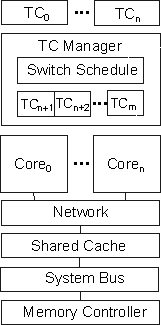
\includegraphics[width=1.08in]{figs/hw_sw_arch.pdf}
%        \caption{The Timing Compartments Architecture}
%        \label{fig:arch}
%    \end{center}
%\end{figure}

%As shown in Figure \ref{fig:arch}, the timing compartments architecture is 
%comprised of a set of $n$ cores which share resources. There is no limitation 
%on $m$, the number of timing compartments that can reside in the system at one 
%time. However, at most $n$ timing compartments can be active (executing on one 
%or more physical cores) at a time. If $m>n$, active timing compartments must 
%occasionally be switched with inactive ones. The TCM addresses this by context 
%switching TCs according to a context switch schedule.

\subsection{Hardware Control Interfaces}

%The hardware protection mechanisms in the previous section need to distinguish 
%memory accesses from different timing compartments.

%\subsubsection{TCIDs}

The hardware protection mechanisms track which timing compartment originated 
each request and handle the requests accordingly. Each core has a register that 
stores the timing compartment ID (TCID) of the TC currently active on that core. This is used to derive 
the tags that are appended to requests originating from that core. The TCID is 
$log\ n$ bits where $n$ is the number of cores in the processor.
Events such as network packets or cache accesses that use shared resources are 
tagged with the TCID of the corresponding core. 
The timing channel protection mechanisms use this TCID to distinguish accesses
from among different timing compartments.

For resource allocation, the hardware protection mechanisms allow the TCM to 
specify which timing compartment can use each partitioned resource.
For example, 
the partitioned cache includes $n$ registers that specify which cache partitions 
can be accessed for each timing compartment. 
%When a request requires a replacement, the cache uses the TCID of the request
%to decide which partitions can allow entries to be replaced according to the
%policy. (Checking is only required on replacements since TCIDs have separate
%address spaces.) 
In the set partitioned cache, the registers specify a mask
that is used to compute the cache array index from the memory address.
The mask maps accesses from each timing compartment to a subset of 
cache sets.
Similarly, each queue at the interface of the shared structures is tagged
with a TCID that owns that queue.
Table~\ref{table:tcid} summarizes the TCID registers in the system.

\begin{table}
\begin{center}
    \begin{footnotesize}
\begin{tabular}{l|l}
    \hline
    Component & TCID Storage \\
    \hline
    Core & $n$ cores. TCID register per core. \\
    \hline
    \multirow{3}{*}{Cache}
    & $n$ response queues. TCID register per queue \\
    & $n$ partition selection registers. \\
    & $n$ MSHR queues. TCID per queue\\
    \hline
    Network & $n$ queues. TCID register per queue\\
    \hline
    \multirow{2}{*}{Memory Controller}
    & $n$ request queues. TCID register per queue \\
    & $n$ response queues. TCID register per queue\\
    \hline
\end{tabular}
    \end{footnotesize}
    \caption{TCID registers for the shared structures.}
    \label{table:tcid}
\end{center}
\end{table}

For time-multiplexed resources, the hardware mechanisms contain control
registers so that the TCM can specify the schedule for time multiplexing.
More specifically, for an $n$-core system, a time-multiplexed resource
uses a schedule with $n$ time slices. Then, for each time slice, control
registers specify the length of the time slice in cycles, and
the TCID that is allowed to use the time slice. Finally, to support
coordination among related components, each time-multiplexed component
allows an offset to be specified by the TCM. The offset determines
the number of cycles before the first time slice starts after a reset.

%Each of the separate MSHR queues are tagged with a TCID of the owner, and 
%requests can only affect the MSHR queues with the same TCID as the request. 
%Each of the time multiplexed resources (the networks, the memory controller, 
%shared cache response ports, and memory controller response ports) have $n$ 
%queues.  Each of these queues has a register to store the TCID which owns that 
%particular queue. A time quantum is scheduled for each queue, so time quanta 
%are allocated to TCs by setting the queue configuration register with the TCID 
%of that TC. A single TC can be granted multiple queues, and therefore, multiple 
%time quanta in each rotation of the schedule. The configuration registers also 
%control the ordering of the queues in the schedule and the time offset of the 
%schedule. The offset delays the start of the schedule by some number of cycles 
%to allow the TDM schedules of multiple devices to be coordinated as described 
%in Section \ref{sec:coordination}. The configuration register can also set the 
%duration of the time quanta for each queue, but this cannot be changed based on 
%the dynamic behavior of the timing compartment.
%\subsubsection{Initialization \& Handling Context Switches}
%The TCM, initializes the system by setting the TCID storage elements listed in 
%Table 1 with the IDs of the initially active timing compartments. At most $n$ 
%of these can be active initially, so if $m>n$, some will be inactive, and the 
%TCM must define a static context switching schedule at initialization time.

\subsection{Context Switches}

% The time between context switches cannot depend on the dynamic behaviour of 
% the TCs. Otherwise, a timing compartment could observe the time that they are 
% context switched in or out to learn information about the timing compartment 
% it is switched with. Instead, context switches occur at a fixed time 
% interval, $T_{CTX}$. Every $T_{CTX}$ cycles the TCM is invoked to replace the 
% timing compartment which has been active the longest with the TC at the head 
% of the inactive TC queue. The compartment which has been switched out is 
% moved to the back of the inactive TC queue.

On a context switch, the TCM sets the TCID of a processing core to reflect
the incoming process (or virtual machine). The TCM also sets the control
registers for each protection mechanism to match the new set of active
timing compartments. Note that changing the resource allocation such as
partition sizes or time-multiplexing schedules may indicate
which process (or VM) is scheduled. However, allocation can be done
independently of data-dependent dynamic behavior (e.g. by allocating resources
based on static performance characterizations). Context switches should not 
depend on process state (e.g. ready or waiting) since process state can be 
data-dependent.

For timing channel protection, the TCM also flushes per-core state elements
during a context switch.
Although private, per-core resources are not concurrently shared by TCs, they 
are shared across context switches. The state modified by the TC that is 
swapped out can affect the timing of the TC that is swapped in.
To perform the context switch, the CPU pipeline and the memory request queue 
are drained. 
%The general purpose registers of the outgoing TC are stored in 
%TCM-space memory and tagged with the TCID. 
The private cache, shared cache 
partition, TLB, and branch predictor state of the outgoing TC are all flushed.  
Finally, the TCID stores of the outgoing TC are replaced with the TCID of the 
incoming TC. 

When switching out a TC with a label that is less than or equal to that of the 
TC that is switched in, flushing is unnecessary. There is no need to prevent 
timing leakage to the new TC since it is permitted by the policy.
Lattice scheduling~\cite{lattice-scheduling} can be applied to reduce the
overhead needed for context switches by scheduling TCs so that their security
labels increase monotonically. 

%The time required to perform a context switch depends on the state and behavior 
%of the outgoing TC. The owner of the incoming TC can observe when the incoming 
%TC begins executing, so this implies a potential leakage of secrets. To 
%prevent this, context switches are bound to always take the worst case time.  
%If a context switch completes early, the incoming TC is stalled until the worst 
%case context switch time has been reached.

%%%%%%%%%%%%%%%%%%%%%%%%%%%%%%%%%%%%%%%%%%%%%%%%%%%%%%%%%%%%%%%%%%%%%%%%%%%%%%%
%% Should mention lattice scheduling
%%%%%%%%%%%%%%%%%%%%%%%%%%%%%%%%%%%%%%%%%%%%%%%%%%%%%%%%%%%%%%%%%%%%%%%%%%%%%%%

\subsection{Handling I/O}
TCs must interact with the TCM to handle requests for I/O without causing a 
timing channel through interaction with a shared OS or hypervisor.
Any resources required to handle I/O requests are allocated in the TC that owns 
them.
Processes that handle I/O are placed in the TC owning the IO 
operation (in a hypervisor environment, I/O processes in the privileged
VM are still placed in the owning TC).
%The process is executed on a core owned 
%by that TC, and similarly, the instructions and data are placed in the 
%address space of that TC.
I/O buffers are allocated for each TC separately. In hypervisor systems such as
Xen\cite{xen-sosp03} which use a shared I/O ring buffer for each VM, a separate
ring buffer must be allocated for each TC (although VMs in the same TC may share
the buffer). 
% Separate, per-TC buffers introduce a minor complication - the OS
% must own a portion of the address space of each TC where these buffers can be
% allocated. Alternately, the buffers can be allocated in user-space (analogously
% within a guest VM) at the discretion of the system designer. 

The instructions that execute a system call or library function will be loaded
into the address space and partitions of the TC that is using them. Often, multiple
copies of the instructions will be loaded in the cache in different partitions.
However, since instructions needn't be written to, there is no coherence issue. 
Although some TCM instructions will reside in different user-space or guest 
TCs, they will still be part of kernel-space processes and can run in 
privileged mode. This is a benefit of separating timing channel protection 
from access controls with timing compartments.

% Placing interrupt handlers in 
% user-space or guest TCs assumes that event timings for the handlers depend
% solely on user-space or guest data. Though this should often be the case, these 
% handlers should be designed to not depend on protected OS or hypervisor data. 
% Writing this software securely is outside the scope of this paper which is 
% primarily focused on hardware mechanisms.

I/O controllers and DMA modules may require additional hardware support to 
remove timing channel protection. Although these are not explicitly described 
in this paper, the general protection approaches described in section
\ref{sec:general_approaches} can be adapted for these devices. For example,
some IO devices can only be used by a single process at a time introducing a
contention based timing channel that can be resolved with time multiplexing.

% Since the TCM allows access controls and timing channel protection to be
% handled separately, the process can be run in privileged mode even though it
% is run in a TC with user-space processes or unprivileged VMs. However, care
% must be taken if the IO operation depends on secrets of both the OS and the
% requesting TC.

%% \subsection{Interprocess and Interdomain Communication}
%% Interprocess communication (IPC) is a feature of most operating systems that
%% allows processes to communicate with one another. Analogously, virtual machines 
%% in a hypervisor system communicate through interdomain communication.
%% % Since 
%% % interprocess and interdomain communication explicitly share information, 
%% % there may be vulnerabilities through these explicit channels, though most
%% % conventional operating systems and hypervisors address this.
%% The time
%% that communication takes place can depend on secrets and create timing channel 
%% vulnerabilities if the program is not written to prevent this. These
%% code-dependent IPC timing channels are best resolved at the language or 
%% software system level.
%% However, even correctly written programs can have IPC timing channels through 
%% hardware.
%% 
%% The most common forms of IPC are shared memory and message passing. With
%% shared memory IPC, the operating system configures a region of memory that can 
%% be accessed by both communicating processes.
%% With message passing, the 
%% processes explicitly send and receive data through system calls. Similar 
%% hardware-level timing channel vulnerabilities exist in each.
%% 
%% Suppose one timing compartment in a shared memory system, 
%% TC1, writes to the shared memory region. The system as described thus far 
%% would use TCID1, the TCID of TC1, to perform the request and would place the 
%% data in the cache partition owned by TC1. TC2, which would like to receive this 
%% data from TC1, must have some way of accessing it. When TC2 reads to this 
%% region, it must get the data from the partition of TC1. This can be done if the 
%% TCM acknowledges the read is for IPC and allows the read from TC2 to be 
%% performed with TCID1. However, since the IPC data is in the same partition as 
%% other data owned by TC1, interference can leak sensitive information to TC2 
%% through a timing channel.
%% 
%% Clearly, IPC operations cannot use
%% either of the communicating compartments directly. This would allow IPC 
%% operations to interfere with any other operations performed by that TC.
%% Instead, the IPC operations are performed in a timing compartment that can be 
%% accessed by each communicating TC. This is 
%% the TC with the security label that is the greatest lower bound (meet) of the 
%% two communicating compartments according to the security policy lattice.  
%% Any network, cache, or memory controller usage while performing IPC operations
%% are done through this meet timing compartment.
%% 
%% Shared memory IPC is implemented by allocating the shared memory space in the 
%% meet TC. Memory requests to the shared space use the network turns and cache 
%% partitions of the meet TC. Message passing IPC is implemented similarly.
%% The meet timing compartment of the sender and receiver is used for both sending
%% and receiving messages.
%% 
%% In some cases, it may be necessary to create a new timing compartment to
%% represent the meet of two communicating compartments rather than to use
%% the meet of the two compartments in the original policy (which may be
%% undesirably accessible to other timing compartments). However, using an 
%% existing TC, if possible, will require less overhead.
%% In either case, it is wasteful to execute IPC operations on a separate core. 
%% Instead, IPC operations are performed on the core that originated them and an OS 
%% trap applies the TCID of the meet TC when using any resource to carry out the 
%% IPC operation.
%% 
%% % An important 
%% % implication of using a TC that is accessed by both communicating parties is 
%% % that the timing of IPC operations is visible to both parties. Any programs 
%% % that use either message passing or shared memory IPC must be written so that 
%% % IPC timings do not leak sensitive information. Though verifying program 
%% % security for timing channels is beyond the scope of this paper, other work has 
%% % explored this topic~\cite{smith-popl98,mitigation1,mitigation2,mitigation3}.
%% 
%% Interdomain communication allows two VMs to communicate, for example, to 
%% emulate a network containing these VMs.
%% Interdomain communication in Xen is based off of grant tables, a data structure 
%% that a domain uses to specify the permissions of other domains to use its 
%% pages. The grant table is shared with Xen, and operated on using hypercalls 
%% (which are similar to system calls, but here a VM requests the hypervisor to 
%% act). To provide timing channel protection, grant tables are allocated in the 
%% meet timing compartment of the communicating domains. The hypercalls must be 
%% implemented so that their timing does not depend on data that the hypervisor 
%% does not want to share with other domains.

% \subsection{Time Slice Coordination (Outline Only)}
% \label{sec:coordination}
% 
% Explain problem without timing details. Use figure that has turn lengths with 
% no offsets. Show a packet traversing through path with latencies outlined and 
% the packet getting delayed. Explain figure.
% 
% Though the l3 hit path is simple, whole l2 miss 
% path is a nontrivial problem - many tradeoffs, used linear 
% optimization. Wrote simulator to explore this. Ultimately found a general scheme
% that an optimizer couldn't beat for the l3 miss path. Finding agood balance between
% the hit and miss paths required an optimizer and we did not find a general scheme
% 
% \subsubsection{L2 Miss Timing Sequence}
% Introduce l3 hit timing sequence with figure. Explain figure.
% 
% Show l3 miss timing sequence. Use figure.
% 
% \subsubsection{Latency Simulator \& Optimal Coordination}
% 
% Explain goal of coordinating (EV of L2 miss latency). Usually achieved by 
% aligning turns of adjacent devices. Use turn lengths (duration a TC is 
% scheduled to use a device - depends time to send message, affects 
% ``randomness'' of schedule) and offsets (difference in start times that
% improves how the schedule relates to the schedule of other devices).
% 
% Show how to optimize l3 hits. Use figure.
% 
% Explain tradeoffs. Use figure?? It is not simple to solve.
% 
% Wrote our own l2 miss (l2 to l2) timing simulator. Explain what it simulates. (Assumes 
% uniform random arrival, calculate latency for every possible arrival in a 
% schedule, gets EV of latency).
% 
% Exhaustive search of L3 hit path. Confirms that an intuitive design is best.
% 
% Cannot exhaustively search L3 miss path latencies. Instead use linear 
% optimizatin. Search space has many relative minima (change offset slightly, 
% suddenly schedule is much better) - cannot use hill climbing. Use simulated 
% annealing. Explain our simulated annealing implementation. Optimize for l3 miss 
% alone and l2 miss latency assuming hit rate of 90\%.
% 
% Tried a scheme we suspected would have a good L3 miss latency. Optimal result 
% was different. Adjusted optimizer result to something that made more intuitive 
% sense and iterated. Reran optimizer on result of iterative approach, and the 
% optimizer could not find a better scheme in 20,000 steps.
% 
% Explain optimal scheme. Use figure.
% 
% For l2 miss latency, no intuitive general approach could be found. Balance 
% between hit/miss paths is difficult.
% 
% 
% \begin{figure}
%     \begin{center}
%         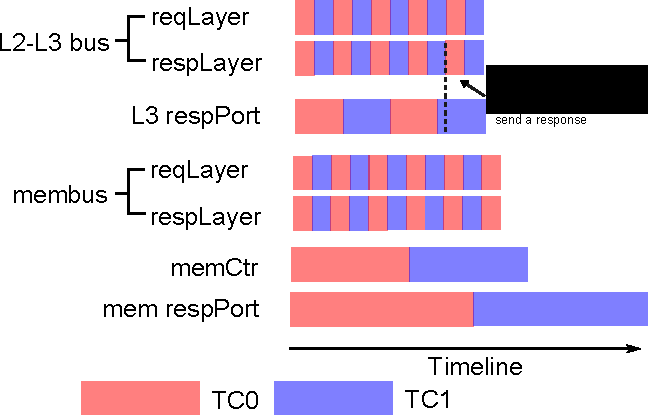
\includegraphics[width=3.46in]{figs/baseline_schedule.pdf}
%         \caption{Cache hit timing sequence.}
%         \label{fig:naive_scheme}
%     \end{center}
% \end{figure}
% 
% 
% \begin{figure}
%     \begin{center}
%         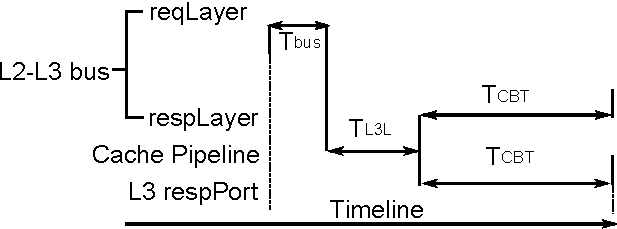
\includegraphics[width=2.4675in]{figs/hit_timing.pdf}
%         \caption{L3 cache hit timing sequence.}
%         \label{fig:hit_timing}
%     \end{center}
% \end{figure}
% 
% \begin{figure}
%     \begin{center}
%         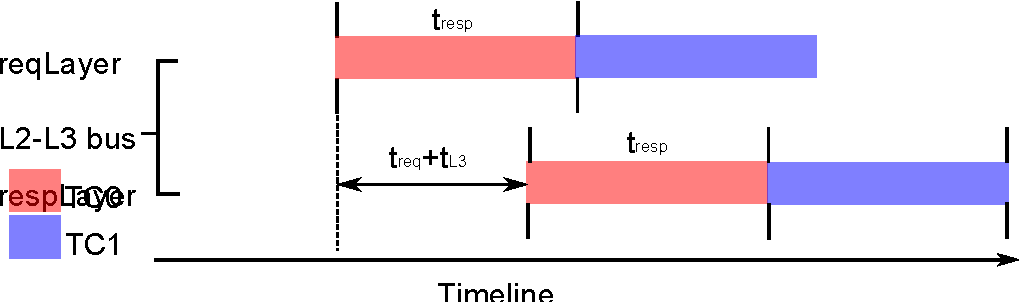
\includegraphics[width=3.2624in]{figs/hit_schedule.pdf}
%         \caption{Cache hit timing path schedule.}
%         \label{fig:hit_schedule}
%     \end{center}
% \end{figure}
% 
% \begin{figure}
%     \begin{center}
%         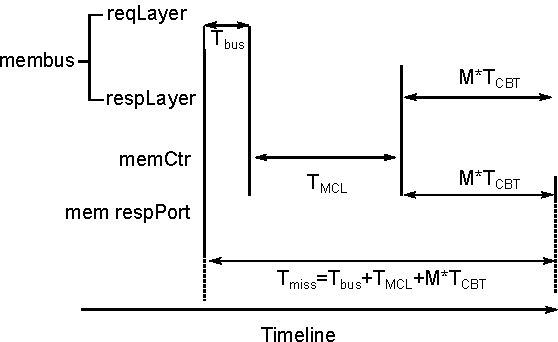
\includegraphics[width=2.9475in]{figs/miss_timing.pdf}
%         \caption{The L3-memory timing sequence.}
%         \label{fig:miss_timing}
%     \end{center}
% \end{figure}
% 
% \begin{figure}
%     \begin{center}
%         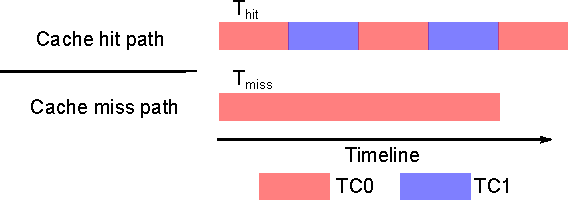
\includegraphics[width=2.9475in]{figs/coordination.pdf}
%         \caption{A coordinated cache miss path schedule.}
%         \label{fig:coordination}
%     \end{center}
% \end{figure}
